\chapter{Contributions}
\label{chap:my-research}

In this chapter, we introduce our contributions to graph learning. The main contributions are in the area of graph structure and structural properties and their role in graph machine learning. Section~\ref{sec:performance-complexity} introduces the performance-complexity trade-off problem, a framework for evaluating models on large graph datasets. Sections~\ref{sec:harp-coarsening} and~\ref{sec:direct-coarsening} present two approaches to graph coarsening based on the aforementioned trade-off paradigm. Section~\ref{sec:CSP} presents our work towards a simple and efficient baseline algorithm for signal propagation in hypergraphs. Finally, Section~\ref{sec:graph-property-effect} introduces our study of the effects of graph properties on downstream task performance.

\section{The performance-complexity trade-off in graph machine learning}
\label{sec:performance-complexity}

One of the key ares of study in our work has been the interplay between graph complexity and the performance of a model used on the graph in question, outlined in \cite{prochazka_scalable_2022, dedic_balancing_2023, dedic_balancing_2024}

The main aim of these works is to explore the performance-complexity characteristics in the context of graph learning. The result of a repeated application of a graph coarsening operation is a sequence of graphs \( G_0, G_1, G_2, \dots, G_L \) where \( G_0 = G \).
Given a model \( M \) that operates on graphs, a performance metric, and a complexity metric, the sequence \( G_0, G_1, \dots, G_L \) corresponds to points in the performance-complexity plane, where advancing along the sequence generally hurts performance and decreases complexity. Denoting $P_i$ performance of model $M$ achieved using the graph $G_i$ with a complexity \( C_i \), our goal can be achieved according to illustration in Figure~\ref{fig:performance-complexity-schema}:
\begin{itemize}
	\item Given maximum available complexity $C_m$, we select such a graph that the complexity of the graph is smaller than $C_m$ and achieve performance $P_3$ -- blue arrows.
	\item Given minimal required performance $P_m$, we select such a graph that $|\mathcal{P}_i|\ge P_m$ with complexity $C_2$ -- green arrows.
\end{itemize}

\begin{figure}
	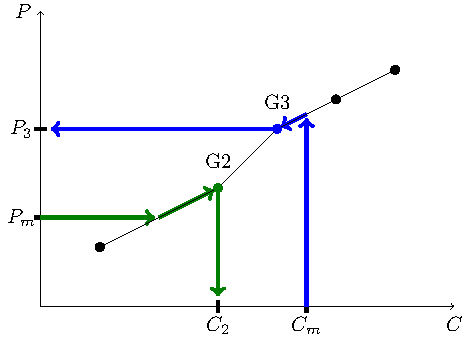
\includegraphics[width=0.7\linewidth]{images/performance-complexity-schema/performance-complexity-schema.pdf}
	\caption{Achieving the target operating point by means of the performance-complexity trade-off. In case of minimal required performance (green arrows), we find the graph $G_2$, where the model achieves at least performance $P_m$. In case of maximal available resources (blue arrows), we select the model achieving performance $P_3$. Original figure from \cite{prochazka_scalable_2022}.}
	\label{fig:performance-complexity-schema}
\end{figure}

This procedure describes a basic way of choosing a \textbf{working point} that is optimal for the particular use-case. The choice of the working point, suitable performance metric and complexity metric are subjective and depend on the particular use-case, downstream task and the environment in which the model is to be deployed. In this work, the transductive node classification accuracy on a testing dataset is chosen as the performance metric. For the complexity metric, the number of nodes in the graph was chosen as it constitutes a good proxy for real-world algorithmic complexity, as shown in \cite{chiang_cluster-gcn_2019}.

\section{A HARP-based method for performance-complexity balancing}
\label{sec:harp-coarsening}

This method builds on the HARP method introduced in \cite{chen_harp_2018} for pretraining methods such as node2vec on coarsened graphs. The sequence \( G_0, G_1, G_2, \dots, G_L \) is generated in HARP consecutively. In an overview, the HARP algorithm first ahead-of-time consecutively coarsens the graph. The method itself can then be executed by repeating the following steps on the graphs from the coarsest to the finest (i.e., from \( G_L \) to \( G_0 \)):
\begin{enumerate}
	\item \textbf{Training on an intermediary graph}. The graph embedding model is trained on \( G_i \), producing its embedding \( \Phi_{G_i} \).
	\item \textbf{Embedding prolongation}. The embedding \( \Phi_{G_i} \) is \textit{prolonged} into \( \Phi_{G_{i - 1}} \) by copying embeddings of merged nodes. \( \Phi_{G_{i - 1}} \) is then used as the starting point for training on \( G_{i - 1} \).
\end{enumerate}

While the prolongation used by HARP is sufficient when used as a means of pre-training, the approach is far too crude when studying the relationship between graph complexity and the quality of graph embedding. In order to overcome this limitation, we present the adaptive prolongation approach. This algorithm works with the pre-coarsened graphs produced by HARP, however, the embedding is learned in a different manner. There are \( K \) prolongation steps (where generally \( K \neq L \)) and each of them uses all graphs \( G_L, \dots, G_0 \). The prolongation steps are driven by local properties of the graph with relation to the downstream task, allowing for different levels of granularity in different parts of the graph. Let us denote \( \Psi_K, \dots, \Psi_0 \) the resulting embedding sequence. The algorithm starts with the coarsest graph \( G_L \), trains a graph model to compute its embedding \( \Psi_K \) and gradually refines it until reaching the embedding \( \Psi_0 \). These prolongation steps are interlaid with continued training of the graph model, as in standard HARP\@. A description of a single prolongation step from \( \Psi_{i + 1} \) to \( \Psi_i \) is schematically outlined in Figure~\ref{fig:adaptive-prolongation} and described in detail in \cite{dedic_balancing_2023}.

\begin{figure}
	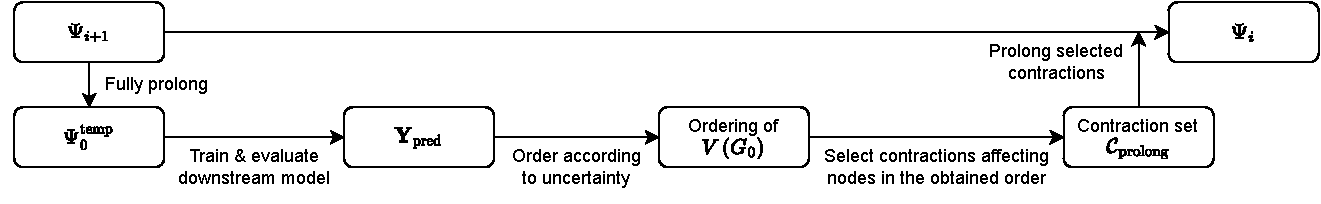
\includegraphics[width=\linewidth]{images/adaptive-prolongation/adaptive-prolongation.pdf}
	\caption{A schematic explanation of the adaptive prolongation algorithm for obtaining the embedding \( \Psi_{i} \) from \( \Psi_{i + 1} \). Original figure from \cite{dedic_balancing_2024}.}
	\label{fig:adaptive-prolongation}
\end{figure}

In \cite{dedic_balancing_2024}, we experimentally evaluated this method on 10 of the most common datasets used for graph machine learning, giving us the performance-complexity curves shown in Figure~\ref{fig:adaptive-coarsening}. The results were further verified using both null hypothesis significance testing as well as the Bayesian Wilcoxon signed-rank test (see \cite{benavoli_bayesian_2014}) with the headline result that at 60\% complexity, the models have over a 99\% probability of being within 10 percentage points of performance on the full graph and at 80\% complexity, they have over 99\% probability of being withing 5 percentage points of performance.

\begin{figure}
	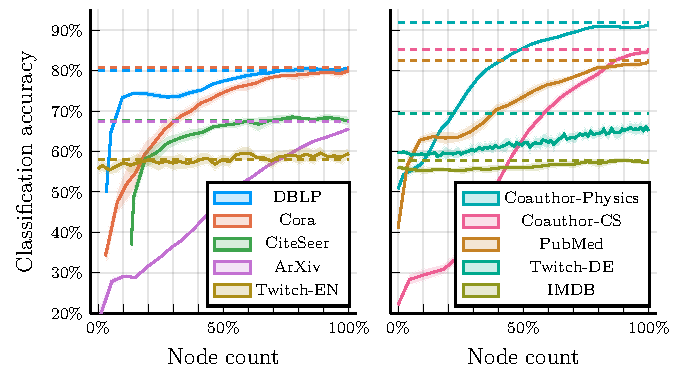
\includegraphics[width=0.8\linewidth]{images/adaptive-coarsening/adaptive-coarsening.pdf}
	\caption{Downstream classifier test-set accuracies at different steps of adaptive prolongation. Dashed line shows the baseline node2vec model accuracy on the full graph. The node count is taken relative to the total node count in each dataset. The results are averaged over multiple runs, with the solid line representing the mean and the shaded area denoting one standard deviation. Original figure from \cite{dedic_balancing_2024}.}
	\label{fig:adaptive-coarsening}
\end{figure}

\section{A direct approach to graph coarsening}
\label{sec:direct-coarsening}

The approach to graph coarsening described in Section~\ref{sec:harp-coarsening} is a two step procedure -- the graph is first repeatedly coarsened and then refined back until reaching an optimal working point. As an alternative to this \enquote{there and back} approach, we proposed a direct approach to graph coarsening in \cite{prochazka_scalable_2022}.

In the direct approach, the sequence \( G_0, G_1, G_2, \dots, G_L \) is generated by the operation of edge contraction, with each graph in the sequence being generated from the previous one by contracting one edge. In the context of this setup, that is, in the situation where we want to apply a GNN on the new graph $G_{i+1}$ and evaluate its performance on the original one ($G_0$), the following issues arise and must be resolved:

\begin{enumerate}
	\item Based on the nodes $v_{X}$ and $v_{Y}$, we need to aggregate training labels (if available) to the new node $v_{XY}$ and decide if this label should be used for training on the coarsened graph, that is to define $\mathvec{y}_{i+1}$ based on $\mathvec{y}_i$.
	\item Apart from labels, node features must be aggregated as well (transforming $\mathcal{X}_i$ into $\mathcal{X}_{i+1}$).
	\item Finally, once we have a prediction for the node $v_{XY}$, we need to establish predictions for all the nodes from $V_0$ that were merged into $v_{XY}$.
\end{enumerate}

To solve the issue of feature aggregation, a simple weighted mean of the features of the contracted nodes is used:
\begin{equation}
	\mathvec{x}_{XY} = \frac{w_X \mathvec{x}_X+w_Y \mathvec{x}_Y}{w_X + w_Y}
\end{equation}
where the weight $w_A$ is given by the number of nodes from the original graph $G_0$ that were merged to $v_A$ in the preceding steps. The same weighted mean operation is used to aggregate training labels (converted to a prior distribution) as well. To solve the issue of refining a prediction of a node \( v_{XY} \) into the predictions of the corresponding nodes in \( G_0 \), a simple copy-paste method is used, meaning all the merged nodes get the same prediction as the combined node.

Finally, the defining idea of \cite{prochazka_scalable_2022} is the order in which the edges are contracted, as this ordering of edges in \( G_0 \) in effect defines the whole sequence \( G_0, G_1, G_2, \dots, G_L \), as shown in Figure~\ref{fig:edge-contraction-sequence}. There exists a theoretical optimal ordering in which nodes with different ground truth labels are never merged until this is no longer possible. Such an optimal ordering gives us an upper bound on the performance-complexity curve and this idea is further explored in the original paper. This optimal ordering is, however, impossible to obtain using training labels only. Instead, we propose to train an auxiliary model on the graph \( G_0 \), use it to obtain a predictive posterior distribution for all of its nodes and then order the edges of \( G_0 \) based on a similarity measure applied to the predictive posterior of the two nodes incident on each edge -- in effect contracting first edges that connect nodes deemed most similar by the auxiliary model. As the auxiliary model, a simple logistic regression was used; cross-entropy and KL divergence were used as the similarity measure. The method was experimentally verified on several publicly available datasets with the results shown in Figure~\ref{fig:direct-graph-coarsening-results}.

\begin{figure}
	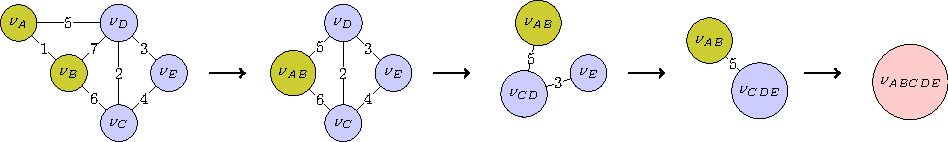
\includegraphics[width=\linewidth]{images/edge-contraction-sequence/edge-contraction-sequence.pdf}
	\caption{Graph sequence determined by a given sequence of edges to contract, where the numbers on edges stand for the edge order for contraction. Original figure from \cite{prochazka_scalable_2022}.}
	\label{fig:edge-contraction-sequence}
\end{figure}

\begin{figure}
	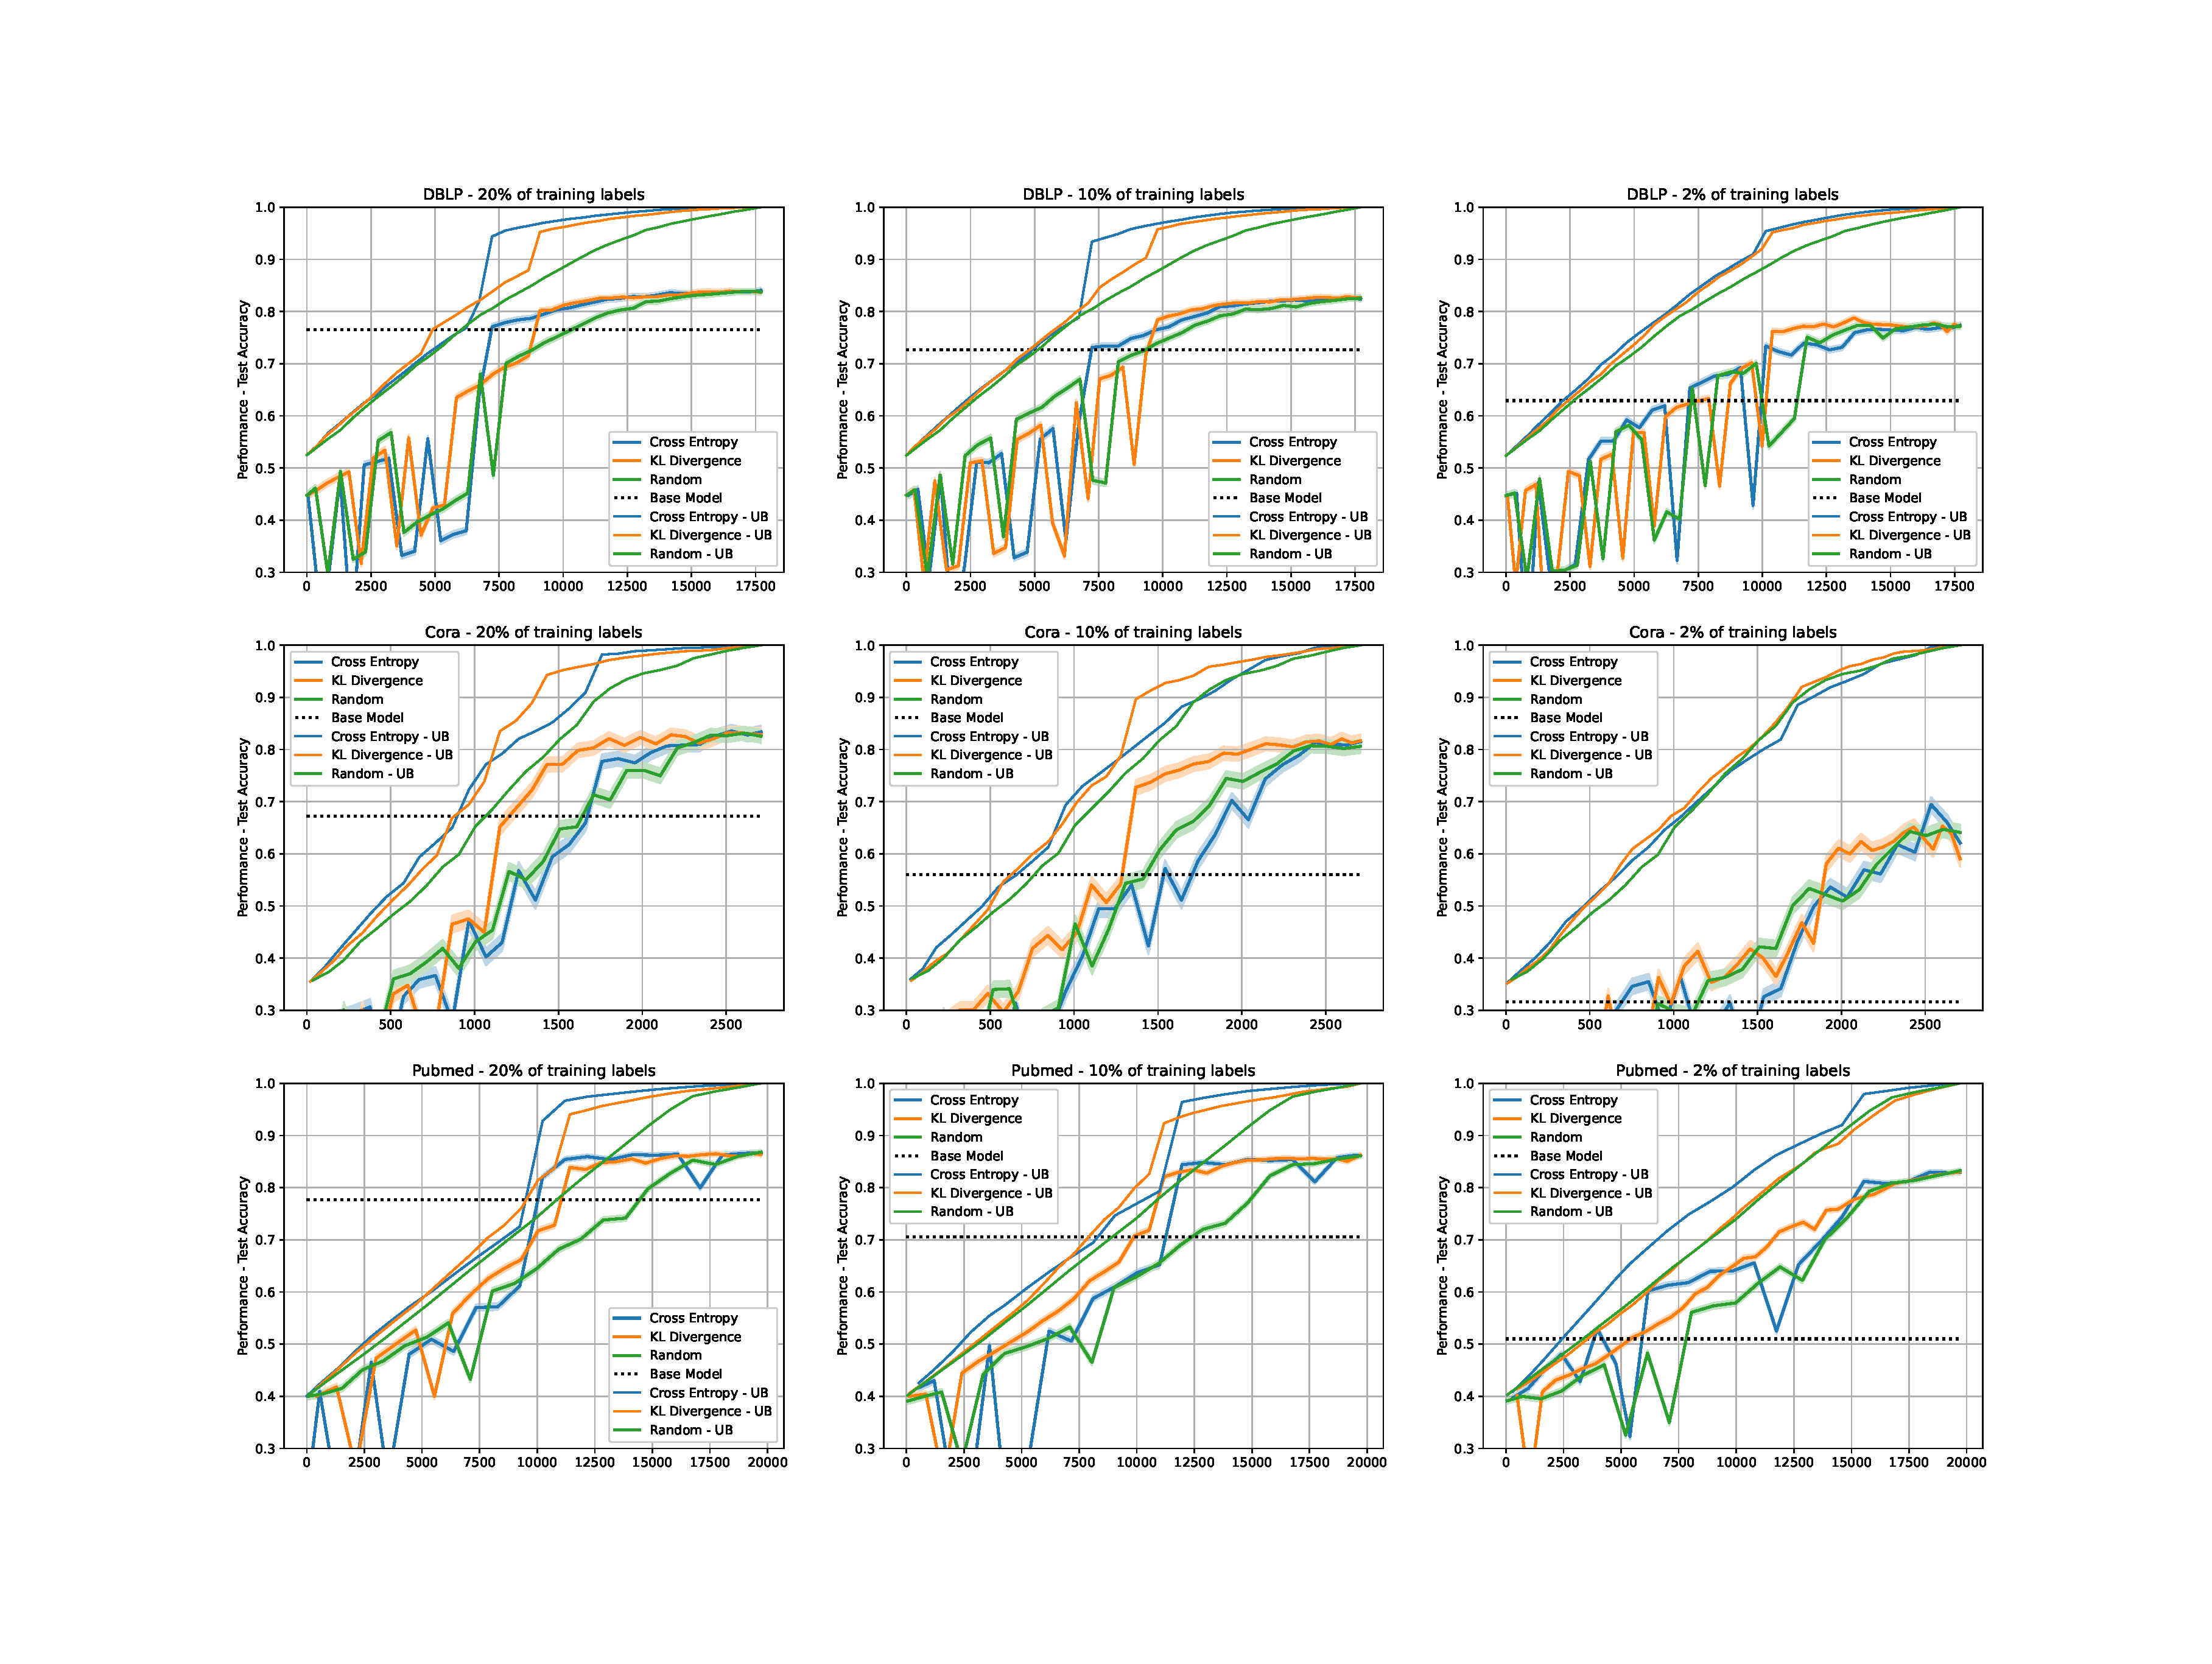
\includegraphics[width=\linewidth]{images/direct-graph-coarsening-results.eps}
	\caption{Performance comparison of various orderings used for sorting the edges for contracting, together with a random ordering. The dependencies are plotted for different number of training labels. The line represents a theoretical upper bound on performance. Original figure from \cite{prochazka_scalable_2022}.}
	\label{fig:direct-graph-coarsening-results}
\end{figure}

\section{A simple, scalable algorithm for signal propagation in hypergraphs}
\label{sec:CSP}

In Section~\ref{sec:performance-complexity}, the performance-complexity trade-off was introduced and subsequently, two approaches to graph coarsening were explored. Simplifying the dataset is, however, only one possible way of tackling the problem of high computational complexity. Another option is to simplify the algorithms themselves so that they may run even on very large datasets. In \cite{prochazka_convolutional_2024}, we introduce \name{Convolutional Signal Propagation} (CSP), a simple and scalable algorithm operating on hypergraphs. CSP has no hyperparameters to tune and is itself a parameter-free method, meaning it doesn't require any training and can be directly applied to a dataset.

We consider for each node in the hypergraph some kind of signal that is to be propagated through the hyperedges. Let the signal be a \( d \)-dimensional vector \( \mathvec{x}_i \) for each node, giving for the whole hypergraph a matrix \( \mathmat{X} \in \mathfield{R}^{n \times d} \). The proposed algorithm propagates this signal $\mathmat{X}$ through the hypergraph $H$. The basic version of CSP consists in a simple averaging of \( \mathmat{X} \) across the hyperedges and nodes of the graph. This averaging can be repeated to obtain smoother final representations, resulting in a multi-step CSP process generating a sequence of representations \( \mathmat{X}^{(l)} \), where \( \mathmat{X}^{(0)} = \mathmat{X} \).

In each step, the representation $\mathmat{X}^{(l)}$ of the nodes is first propagated to the hyperedges to obtain their representations 
\begin{equation}\label{eq:CSP-edge-score}
\mathvec{r}_j^{(l)}=\frac{1}{\edeg \left( e_j \right)}\sum_{\substack{i \\ v_i\in e_j}} \mathvec{x}_i^{(l)} 
\end{equation}
that is the average of the representation of the individual nodes contained in the hyperedge. In the second step, this hyperedge representation is propagated again into nodes:
\begin{equation}\label{eq:CSP-node-score}
\mathvec{x}_k^{(l+1)}=\frac{1}{\mathdeg \left( v_k \right)}\sum_{\substack{j \\ v_k \in e_j}} \mathvec{r}_j^{(l)}.
\end{equation}

The steps~\ref{eq:CSP-edge-score} and~\ref{eq:CSP-node-score} constitute the proposed Convolutional Signal Propagation algorithm, which can be summarily written as
\begin{equation}\label{eq:CSP-one-node}
    \mathvec{x}_k^{(l+1)} = \frac{1}{\mathdeg \left( v_k \right)}\sum_{\substack{j \\ v_k \in e_j}} \frac{1}{\edeg \left( e_j \right)}\sum_{\substack{i \\ v_i \in e_j}} \mathvec{x}_i^{(l)}.
\end{equation}
We establish a diagonal node-degree matrix \( \mathmat{D}_v \in \mathfield{N}^{n \times n} \) with \( (\mathmat{D}_v)_{i,i} = \mathdeg \left( v_i \right) \) and \( (\mathmat{D}_v)_{i,j} = 0 \) for \( i \neq j \). Analogously, the hyperedge-degree matrix is a diagonal matrix \( \mathmat{D}_e \in \mathfield{N}^{m \times m} \) with \( (\mathmat{D}_e)_{i,i} = \edeg \left( e_i \right) \) and \( (\mathmat{D}_e)_{i,j} = 0 \) for \( i \neq j \). Equation~\ref{eq:CSP-one-node} can then be rewritten into the matrix form
\begin{equation}
    \mathmat{X}^{(l+1)} = \mathmat{D}_v^{-1} \mathmat{H} \mathmat{D}_e^{-1} \mathmat{H}^T \mathmat{X}^{(l)}.
\end{equation}

This CSP algorithm is very simple and can be efficiently implemented in a few lines of Python code or even as a single SQL query (see \cite{prochazka_convolutional_2024} for code). This apparent simplicity hides the fact that CSP is closely related to several established algorithms on graphs. We show that CSP applied to a feature matrix corresponds to a single layer of hypergraph convolution (see \cite{bai_hypergraph_2021}) with parameter matrices replaced with \( \mathmat{I} \). If instead a masked version of the label matrix is used as the signal \( \mathmat{X} \), CSP is equivalent to the label propagation algorithm (see \cite{zhu_learning_2003}). When the incidence matrix is used as the signal (i.e. \( \mathmat{X} = \mathmat{H} \)), the resulting algorithm is variant of a multinomial Naive Bayes classifier.

The CSP algorithm was experimentally verified on 8 multigraph datasets in both a classification setting as well as a retrieval setting. Three variants of CSP (with 1, 2 or 3 layers) were compared to a Naive Bayes classifier, a random forest classifier, a logistic regression model and a Hyper-Conv model from \cite{bai_hypergraph_2021}. The main result is that CSP was in the vast majority of scenarios withing 5 percentage points of the best model (sometimes CSP was the best model). At the same time CSP was (apart from one dataset) the computationally most efficient algorithm, with Hyper-Conv (the state-of-the-art GNN model for hypergraphs) being approximately four orders of magnitude slower. In summary, we have shown that a relatively simple, fast, parameter-free method may serve as an efficient baseline model for tasks on hypergraphs.

\section{The effect of graph properties on downstream task performance}\label{sec:graph-property-effect}

While typically in graph machine learning, the graph itself is taken as a given, in practice, this may not be the case and the question of how to transform the available data into a graph may affect the performance of the downstream task in a profound way. This problem is the motivation behind our work reported in \cite{prochazka_which_2023}. Given the complex and multi-faceted nature of this problem, we limited ourselves to the sub-problem of measuring and predicting the suitability of a given graph representation to a given downstream task.

To solve this problem, we first represented the graph dataset by its \emph{properties}, that are aggregate values representing the whole graph dataset instead of individual nodes or edges. A GNN model \cite{hamilton_inductive_2017} was trained to solve the task, and its performance is measured using several metrics. The main aim of this work was to extract information about the usefulness of individual graph properties from a \emph{meta-model} that is trained on the graph dataset properties to predict the GNN performance represented by the \emph{performance metrics}.
In the reported research, we proposed and evaluated such a meta-model on publicly available datasets, however, it forms a useful and general tool for evaluating the suitability of graph datasets to tasks on them, which is a basic prerequisite to solving the more general problem of constructing an advantageous graph representation.

In total, we used 17 different graph properties, ranging from simple ones like node count and the ratio between different classes, standard properties used for describing graphs such as the average node degree, properties relating specifically to graph machine learning such as global assortativity and node, edge and class homophily and finally ending with some custom properties defined by us specifically for this work. We specifically chose this list of properties such that some of them are aware of the downstream task (i.e.\ labels), some take into account the graph structure and some operate on the features associated with the nodes of the graph.

We used 7 different publicly available datasets and for datasets with multiple classes, we considered each of the classes as a separate binary classification problem independently, giving us a total of 139 different binary graph classification problems. For each of these 139 problems, we trained a GraphSAGE model and evaluated it using 5 different performance metrics. This list of graph properties together with the associated model performance metrics gives us a dataset to train the meta-model on. As the focus in the meta-model is on simplicity and explainability, a random forest regression model was used for this task, taking a third of the 139 data points as training data. The meta-model was experimentally verified to be a sufficiently good predictor of the model performance from the graph properties. Subsequently, the meta-model was used used to give an explanation of the importance of the various graph properties to the GNN performance using Shapley Additive Explanations (SHAP, see \cite{shapley_notes_1951}). The results of this experiment for the log-loss performance metric are shown in Figure~\ref{fig:graph-property-importance}. Overall the results vary between the different performance metrics, however, some universal rules can be observed, such as higher homophily (in all its variants) leading to better performance.

\begin{figure}
	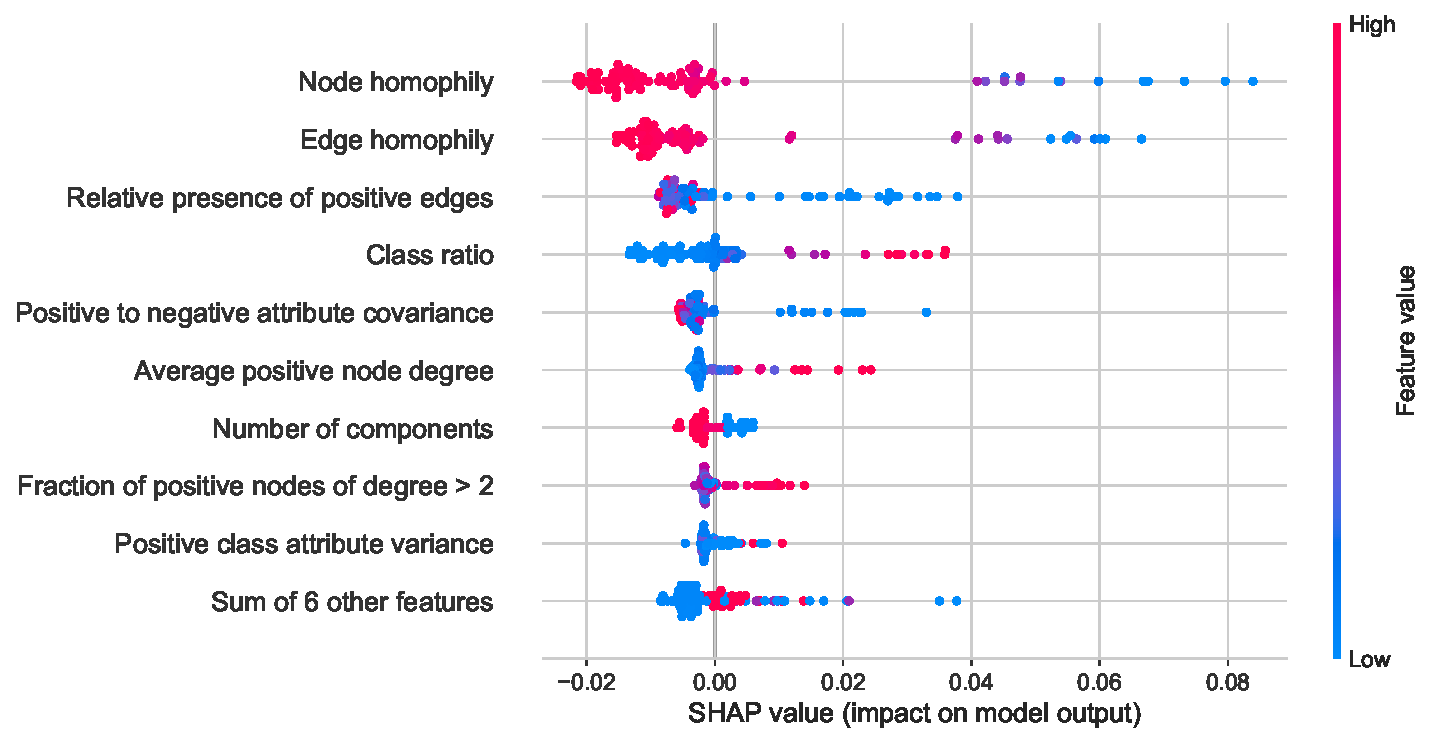
\includegraphics[width=\linewidth]{images/graph-property-importance.pdf}
	\caption{SHAP explanation for log loss prediction identifying node and edge homophily as the most important graph properties for the log-loss prediction. Therefore, we claim these graph properties to be the most important graph properties, when training GNN on the graph with log-loss objective. In addition, the SHAP explanation shows that the higher homophily the lower log-loss and therefore the better performance. Recall that the GNN aims to minimize log-loss. Original figure from \cite{prochazka_which_2023}.}
	\label{fig:graph-property-importance}
\end{figure}

Apart from measuring the importance of different graph properties, the meta-model was also used to predict optimal values of hyperparameters for the underlying GraphSAGE model. This idea will be further described in Section~\ref{sec:gnn-hpo}.
